\documentclass[a4paper, 12pt]{report}

\usepackage[utf8]{inputenc}
\usepackage[usenames,dvipsnames,svgnames,table]{xcolor}
\usepackage[marginparwidth=28mm]{geometry}
\usepackage[pdftex]{graphicx}
\usepackage{tikz}

\usepackage{filecontents}
\usepackage[T1]{fontenc}
\usepackage[UKenglish]{babel}
\usepackage{newpxtext,newpxmath}
\usepackage[babel=true]{csquotes}
\usepackage[round]{natbib}
\usepackage[colorinlistoftodos]{todonotes}
\usepackage{comment}
\usepackage{tikz}
\usetikzlibrary{arrows,automata}
\usepackage{ccaption}

% Logos
\newcommand{\ulb}{
\includegraphics[scale=1.1]{PageDeGarde_MFE/logo_ULB2.pdf}}
\newcommand{\polytech}{
\includegraphics[scale=0.35]{PageDeGarde_MFE/logo_polytech_FR.pdf}}

% Polices
\definecolor{ULBblue}{rgb}{0,0.2196,0.5765}
\newcommand{\fontTitle}{\sffamily \Huge\selectfont \color{ULBblue}}
\newcommand{\fontSubtitle}{\sffamily \LARGE \selectfont \color{ULBblue}}
\newcommand{\fontText}{\sffamily \selectfont}
\newcommand{\fontColor}{\sffamily \selectfont \color{ULBblue}}

% Titre
\newcommand{\titleA}{\fontTitle{Human - Robots Swarms Interactions}} % Titre identique au titre remis au secrétariat
%\newcommand{\titleB}{\fontTitle{Deuxième ligne de titre du mémoire}} % (dans la langue de rédaction a priori)
% Sous-titre
\newcommand{\subtitle}{\fontSubtitle{Ligne du sous-titre du mémoire}}
% Titre du diplôme
\newcommand{\diplomaA}{\fontText{Mémoire présenté en vue de l’obtention du diplôme}} % A laisser en Français
\newcommand{\diplomaB}{\fontText{d'Ingénieur Civil en Informatique à finalité Intelligence Computationnelle}}

% Etudiant
\newcommand{\student}{\textbf{\sffamily \large Anthony Debruyn}}

% Supervision
\newcommand{\promAa}{\fontColor{Directeur}}
\newcommand{\promAb}{\fontText{Professeur [Prénom Nom]}}
\newcommand{\promBa}{\fontColor{Co-Promoteur}}
\newcommand{\promBb}{\fontText{Professeur [Prénom Nom]}}
\newcommand{\promCa}{\fontColor{Superviseur}}
\newcommand{\promCb}{\fontText{[Prénom Nom]}}
\newcommand{\deptA}{\fontColor{Service}}
\newcommand{\deptB}{\fontText{[Nom du service]}}

% Année académique
\newcommand{\yearA}{\fontColor{Année académique}}
\newcommand{\yearB}{\fontText{2014 - 2015}}

%%%%%%%%%%%%%%%%%%%%%%%%%%%%%%%%%%%%%%%%%%%%%%%%%%%%%%%
% MY NEW COMMANDS
%%%%%%%%%%%%%%%%%%%%%%%%%%%%%%%%%%%%%%%%%%%%%%%%%%%%%%%

\newcommand{\quoto}[2]{
\begin{quotation}
\begin{it}
\enquote{#1} - #2
\end{it}
\end{quotation}
}

\newcommand{\quot}[1]{\textit{\enquote{#1}}}


\newcommand{\epuck}[3][0] % [angle]{x}{y} avec angle optionel
{
	\draw [very thick, fill=white] (#2,#3) circle [radius=0.5];
	\draw [very thick, rotate around={#1:(#2,#3)}] (#2-0.25,#3-0.433) -- (#2,#3+0.45) -- (#2+0.25,#3-0.433);
}

\newcommand{\human}[3][0] % [angle]{x}{y}
{
	\draw [line width=1.5pt, rotate around={#1:(#2,#3)}] (#2,#3+1) -- (#2-0.866,#3-0.5) -- (#2+0.866,#3-0.5) -- cycle;
	\draw (#2,#3) node[scale=2, rotate around={#1:(#2,#3)}]{H};
}

%%%%%%%%%%%%%%%%%%%%%%%%%%%%%%%%%%%%%%%%%%%%%%%%%%%%%%%
% NEW STYLES
%%%%%%%%%%%%%%%%%%%%%%%%%%%%%%%%%%%%%%%%%%%%%%%%%%%%%%%

\captiondelim{ -- }
\captionnamefont{\small\sf\bfseries}
\captiontitlefont{\small\sf}
\precaption{\rule{\linewidth}{0.4pt}\\}
\setcounter{secnumdepth}{3}
\setcounter{tocdepth}{3}

%%%%%%%%%%%%%%%%%%%%%%%%%%%%%%%%%%%%%%%%%%%%%%%%%%%%%%%
% THE DOCUMENT
%%%%%%%%%%%%%%%%%%%%%%%%%%%%%%%%%%%%%%%%%%%%%%%%%%%%%%%

\begin{document}

	\thispagestyle{empty}
	\newgeometry{top=2.5cm, bottom=1.5cm, left=2.5cm, right=1cm}
	\setlength{\unitlength}{1mm}
	\noindent\begin{picture}(175,257)
	
		\put(0,245){\polytech}
		\put(153,139.5){\ulb}
		
		\put(8,155){\makebox(150,10)[l]{\titleA}}
%		\put(8,145){\makebox(150,10)[l]{\titleB}}
		\put(8,135){\makebox(150,10)[l]{\subtitle}}
		
		\put(0,75){
		\begin{tikzpicture}[scale=0.1]
		\fill [fill=ULBblue](0,0) rectangle (0.8,90);
		\fill [fill=ULBblue](0,57) rectangle (152,57.8);
		\end{tikzpicture}}
		
		\put(8,120){\makebox(150,5)[l]{\diplomaA}}
		\put(8,115){\makebox(150,5)[l]{\diplomaB}}
		
		\put(8,75){\makebox(150,10)[l]{\selectfont \student}}
		
		\put(8,44){\makebox(80,5)[l]{\promAa}}
		\put(8,39){\makebox(80,5)[l]{\promAb}}
		\put(8,31){\makebox(80,5)[l]{\promBa}} % Commenter la ligne si pas nécessaire
		\put(8,26){\makebox(80,5)[l]{\promBb}} % Commenter la ligne si pas nécessaire
		\put(8,18){\makebox(80,5)[l]{\promCa}} % Commenter la ligne si pas nécessaire
		\put(8,13){\makebox(80,5)[l]{\promCb}} % Commenter la ligne si pas nécessaire
		\put(8,5){\makebox(80,5)[l]{\deptA}}
		\put(8,0){\makebox(80,5)[l]{\deptB}}
		
		\put(145,5){\makebox(30,5)[r]{\yearA}}
		\put(145,0){\makebox(30,5)[r]{\yearB}}
	
	\end{picture}
	\restoregeometry
	
% Template conçu par Benjamin Vanhemelryck et revu par François Bronchart - Mai 2013
	
%%%%%%%%%%%%%%%%%%%%%%%%%%%%%%%%%%%%%%%%%%%%%%%%%%%%%%%
% TABLE OF CONTENT
%%%%%%%%%%%%%%%%%%%%%%%%%%%%%%%%%%%%%%%%%%%%%%%%%%%%%%%

\tableofcontents
\listoftodos
	
%%%%%%%%%%%%%%%%%%%%%%%%%%%%%%%%%%%%%%%%%%%%%%%%%%%%%%%
% TEXT
%%%%%%%%%%%%%%%%%%%%%%%%%%%%%%%%%%%%%%%%%%%%%%%%%%%%%%%

\chapter{Introduction}

[To write at the end. When I have a global view.]

\chapter{The Problem}
	\section{Introduction}
	
	In this section, we will discuss the problem that led to the creation of this thesis by first providing the reader with some general insight in the world of swarm robotics and swarm intelligence. Then we will focus on specific parts of these domains of study: design methods, feedbacks between human and robots' swarm. Eventually, we will conclude with the main problem this thesis is trying to solve.
	
	\section{Swarm Engineering}
	
	This section and the next one are largely inspired by~\citet{brambilla2013swarm}, a reviewing article on swarm engineering. For \citet{csahin2005swarm}, swarm robotics is defined as \quot{the study of how large numbers of relatively simple physically embodied agents can be designed such that a desired collective behavior emerges from the local interactions among agents and between the agents and the environment}~\citep{csahin2005swarm}. Swarm robotics can be separated from other robotic studies by the following characteristics \citep{brambilla2013swarm}:
	
\begin{itemize}
\item Robots are \emph{autonomous}
\item Robots evolve \emph{in the environment} and can interact with it
\item Robots' interactions are \emph{local} (sensors and communications)
\item No \emph{centralised control} or \emph{global knowledge}
\item Robots \emph{cooperate} to achieve a certain goal
\end{itemize}

As in this field of study, one is always looking for \emph{robust}, \emph{scalable} and \emph{flexible} systems, the main source of inspiration is the group of social animals: ants, birds, fishes, ... When some of these simple animals gather in groups, they are able to perform tasks that could not be achieved individually (collective behaviour emerges from local interactions). Below are listed the definitions of these three terms \citep{brambilla2013swarm}:

\label{def:robustness_scalability_flexibility}
\begin{description}
\item[Robustness:] Resistance against \emph{loss of group entities}. One can increase it by adding redundancy or remove the need for a leader.
\item[Scalability:] Low variation in the performance of a system with respect to the \emph{size of the system}. It can be increased by encouraging local interactions, such as sensing and communications.
\item[Flexibility:] Low variation in the performance of a system with respect to the \emph{type of environment or the task}.
\end{description}

With these definitions in mind, we can explain swarm engineering as:

\quoto{Swarm engineering is an emerging discipline that aims at defining systematic and well founded procedures for modeling, designing, realizing, verifying, validating, operating, and maintaining a swarm robotics system.}{\cite{brambilla2013swarm}}

\citet{kazadi2000swarm} points out that \quot{to the swarm engineer, the important points in the design of a swarm are that the swarm will do precisely what it is designed to do, and that it will do so reliably and on time} \citep{kazadi2000swarm}.
	
	\section{Design Methods}
	
	\citet{brambilla2013swarm} did a pretty good job in classifying the different methods to design swarm robotics systems. Design is the period of time that starts at the definition of the requirements and specifications, and ends with the development. They divide the methods into two categories: \emph{behaviour-based design}, and \emph{automatic design}.
	
		\subsection{Behaviour-based Design}
		\label{sec:behaviour_based_design}
		
		All methods in this group mean developing the solution by hand. No learning or automatic tool was used to arrive at an accepting collective behaviour. This is associated with a trial and error process, and involves a lot of tuning. This is the kind of procedure that people usually implement. \citeauthor{brambilla2013swarm} subdivided this group into 3 categories: \emph{probabilistic finite state machine design}, \emph{virtual physics-based design} and \emph{other design methods}.
		
			\subsubsection{Probabilistic Finite State Machine Design}
			
			PFSMs \citep{minsky1967computation} are one of the most used methods to create collective behaviours. As the robots need to take decisions based on their readings and current state, they constitute an intuitive choice. Each transition is characterised by a probability to follow that transition. The value can be fixed or variable, in which case it will generally depend on the current state of the system. One example of such a variable value is the \emph{response threshold} found by \citet{granovetter1978threshold} (also \citet{bonabeau1997adaptive}) \todo{Add figures}.
			
			\subsubsection{Virtual Physics-Based Design}
			\label{sec:virtual_physics}
			
			The next subcategory takes physics laws as a model to generate behaviours. Robots are assimilated to virtual particles under the influence of virtual potential fields and virtual forces. The robots compute the total force by summing all the forces associated to each influence in the system:
			$$\overline{F} = \sum_{i}{\overline{f_i}} ~\mbox{, where $\overline{f_i}$ is a virtual force.}$$
			$\overline{f_i}$ can be expressed in polar coordinates: $$\overline{f_i} = f_i(d_i)e^{j\theta_i}.$$ 
			One of the most used virtual potentials is the Lennard-Jones potential whose utility is to keep a robot at a certain distance\todo{Figure}: 
			$$ f(d) = \epsilon \left[ \left(\frac{\sigma}{d}\right)^{12} - 2 \left(\frac{\sigma}{d}\right)^6 \right]$$, where $\epsilon$ is the gain, $\sigma$ is the target distance and $d$ is the current real distance. 
			This method is very appealing thanks to the absence of multiple rules, states, and tests to decide which actions to execute. Only one mathematical formula translates the inputs into outputs for the actuators, in a smooth and elegant way. Multiple behaviours can be combined by simply summing the corresponding resulting vectors \citep{brambilla2013swarm}. As this method is based on the laws of physics, it is often used when a robot formation is needed.
			
			\subsubsection{Other Design Methods}
		
			Other methods not belonging to the two previous sections can also be cited. Among them, a scripting language created by \citet{bachrach2010composable}: \emph{Protoswarm}. The language allows one to code for the group, and not for the individual, easing the design of the system.
		
		\subsection{Automatic Design}
		
		With automatic design, the generation of the behaviours is left to the computer. No real intervention from the developer is needed \citep{brambilla2013swarm}. \citeauthor{brambilla2013swarm} subdivide again the main category into subcategories: reinforcement learning, and evolutionary robotics and others (which we will not talk about).
		
			\subsubsection{Reinforcement Learning}
			
			Through reinforcement learning, the agent can learn the target behaviour with a trial and error procedure. Positive feedback is returned if the resulting behaviour is close to the target one, and negative feedback is returned if it is far from it. Iteratively, the robot (or agent in a simulation) will come closer to the wanted behaviour (optimal policy) by trying to maximise the rewards received from the environment. Although it may look interesting on paper, designers would need to overcome some difficulties. One of them is called \emph{spatial credit assignment}: since the swarm gets the reward at the end of the experiment, how can we manage to turn it into individual rewards? Indeed, the learning is at the individual level, not at the collective level \citep{wolpert1999introduction}.
			
			\subsubsection{Evolutionary Robotics}
			
			Evolutionary robotics are based on the Darwinian principle of natural selection and evolution. At the beginning of the learning process, a population of individual behaviours is generated randomly. For each generation of the population, a few experiments are run with each individual behaviour. This means the behaviour is used by the entire group of agents. A fitness is computed on basis of the collective performance. At the end of all the experiments, the best individual behaviours in the population are kept and may undergo some changes, like mutation or cross-over. Generations over generations, the behaviours in the population move towards the target collective behaviour. Most of the time, this method is associated with neural networks whose parameters are iteratively adjusted. This whole learning process is computationally intensive and does not guarantee its convergence. Furthermore, the complexity of the final behaviours is relatively low. Usually the same behaviours can be obtained by using behaviour-based design \citep{brambilla2013swarm}.
			
	\section{Analysis}
	
	To check that the system verifies certain properties and exhibits the target behaviour, the swarm engineer has to go through the analysis process, usually by means of models. One can classify the models into 2 levels: \emph{the microscopic level}, and \emph{the macroscopic level} \citep{brambilla2013swarm}. The first one considers the individuals constituting the group, and their interactions. The second one focuses on the group itself and its characteristics. Managing to find a model comprising both levels, microscopic and macroscopic, is very challenging \citep{abbott2006emergence}. This is why most of the works only focus on one of the two aspects.
	
		\subsection{Microscopic Models}
		
		The level considered here describes the entities composing the group, their interactions between one another, and with the environment (their behaviour, see section \ref{sec:behaviour_based_design}) in \emph{simulations}. The amount of detail in the model can vary from representing robots as point-masses to 3D worlds with advanced physics and accurate representation of the sensors and actuators. Most of the simulators for swarm robotics systems do not offer a great scalability, i.e., they do not perform well with very large groups of agents. This is problematic since large numbers are common in this field of study. To address this issue, \citet{pinciroli2012argos} developed a simulator (ARGoS) which allows experiments with more than $10^5$ robots in real time \citep{brambilla2013swarm}.
		
		\subsection{Macroscopic Models}
		
		The system is here studied at a higher level, not viewing the group as composed of agents, but as a single entity. In this category, works can use \emph{rate or differential equations}, \emph{classical control and stability theory} or other mathematical framework \citep{brambilla2013swarm}.
		
		\subsection{Real-robot Analysis}
		
		Experiments with real robots allow the developer to assess the performance of the system under real conditions for the sensors and actuators, which are somehow idealised in the simulators or the other models. It should not be used to validate the behaviours in real-world applications, as the arena environment in which the robots evolve is heavily controlled (light intensity, landscape, interferences). Therefore, it should be viewed as a way to include realistic noise patterns in the experiments \citep{brambilla2013swarm}.
	
	\section{Human - Robot Interaction}
	
	\todo[inline]{Necessary?}
	
	\section{Human - Robots Swarm Interaction}
	
	Human - Robotic swarm interaction is the study of how humans can interact with a swarm to control it and receive feedback from it \citep{brambilla2013swarm}. A proper feedback is needed by the operator in order to make the right decisions. Since swarms must ideally be autonomous and make decisions in a distributed way, it is difficult to insert a communication with a human operator in the system to gain control.\\
	
	Currently, little attention has been devoted to the study of the interaction between humans and robotic swarms, how one can send instructions and receive feedback. People investigating in the field encounter many difficulties, such as the difference of perspective between the swarm and the human operator (the human only observes the global collective behaviour, not the local interactions or individual behaviours driving the robots), the simplicity of the hardware found on the robots, or the efficient synthesis of all the information sent by the robots. All the existing types of interactions in the literature present a major disadvantage: they require an extra layer between the group of robots and the human. This requirement might not always be satisfied when we remember that swarms like this are mostly destined to evolve in an unknown environment. The monitoring equipment necessary to operate the swarm may not be safely deployed. Furthermore, a synthesis of all the local information pieces must be done in order to provide an understandable state of the system to the human. A supplementary step that involves modelling, additional overheads and perhaps heavy computations, and the gathering of all information at a central point (eliminating by the way the distributed and not centralised properties of the swarm system) \citep{podevijn2012self}.\\
	
	\citet{daily2003world} used a head-mounted display and augmented reality to add information right on top of the robot in the environment itself, suppressing the need for an additional display. \citet{baizid2009human} proposed a platform to interact with multiple robots simultaneously through a graphical user interface, or a head-mounted display, virtual reality etc. They also studied how virtual reality abstraction affected the human perception and cognitive capabilities, i.e, they created a virtual environment by filtering useless information. \citet{mclurkin2006speaking} developed an centralised graphical user interface taking inspiration from real-time strategy video games, where one must control armies. They also imagined a feedback approach based on LEDs and sounds. The robots transmit their internal state by applying to their LEDs and sound system a defined pattern, recognisable by the operator, now able to quickly understand the state of the swarm without looking at a supplementary interface.
	
	\citet{podevijn2012self} argue that self-organised mechanism, as those ruling the behaviour of the swarm, should be used to provide feedback to the operator. They suggest that the best entity which could communicate the status of the system and the whole swarm is the swarm itself. They performed experiments using colour feedback to distinguish different internal states and split the swarms into groups to tackle different tasks.\\
	
\begin{comment}
[Currently, only little research on feedback between human and robots swarms. That research is focused on interaction with an additional layer... Mostly unidirectional communication (human to robots). Need new types of interactions for new applications. Robots to human (guide). Write about article saying self-organised feedback is better.] \todo{Remove}
\end{comment}


	\section{Protection and Exploration}
	
	As swarm robotic systems are mostly destined to operate on risky floors, unknown environment, it would seem logical to consider their application in exploration and/or protection missions. However, at the time of writing this thesis, we could not find any study on the subject. Exploration experiments never included a human, or other living organism. The object of this thesis is to address this lack of study by designing and implementing a protective behaviour executed by a robotic swarm.
	
	The human operator is here part of the swarm system. The swarm has to protect him by preventing him from going into dangerous areas, in the same way a group of bodyguards protects someone. The swarm has to follow the operator anywhere to ensure permanent protection.\\
	
	We believe this work to be important since it could lay the foundations of a new branch in swarm engineering: human protection, escort or swarm turn-by-turn navigation.

\chapter{Solution}

	\section{Introduction}
	
	This section details the solution to the given problem and all the choices that resulted in it. The explanation will take a top-down approach, first reviewing the general and early choices faced (as early choices mean general choices). It will then go deeper in the details.
	
	\section{Swarm Robotics}
	
	The first question one could ask is: why swarm robotics for such an application? The answer to that question lays in section \ref{def:robustness_scalability_flexibility}. Robustness, scalability and flexibility are characteristics that make swarms of robots really interesting in unknown environments \citep{brambilla2013swarm}.\todo{Insert justification?} In case one of the agents is broken, we do not want to see the whole system collapse and leave the human unattended. Flexibility guarantees that the solution will work in different conditions, environments, which is an advantage for exploration. In case of loss of robots, scalability would maintain the protection.
	
	\section{The Shape}
	
	The first step of the thesis is the design of the solution, to imagine how the system will look like and how we will implement it. The first choice faced was the overall behaviour of the swarm. How do the robots move around the human? What shape will they try to respect? This choice is important because it will define the overall look of the system.\\
	
	The first shape that intuitively comes in mind is the circle. The circle is the most elementary shape in geometry. It offers the best ratio:
	$$\frac{\mbox{Surface}}{\mbox{Perimeter}} = \frac{r}{2}~\mbox{, where r is the radius of the circle.}$$
	
	That means that fewer robots are needed for the same protected area, and more space for the human with a certain amount of robots. Luckily, it is also the easiest shape to realise in practice.
	
	\begin{figure}[!h]\centering
	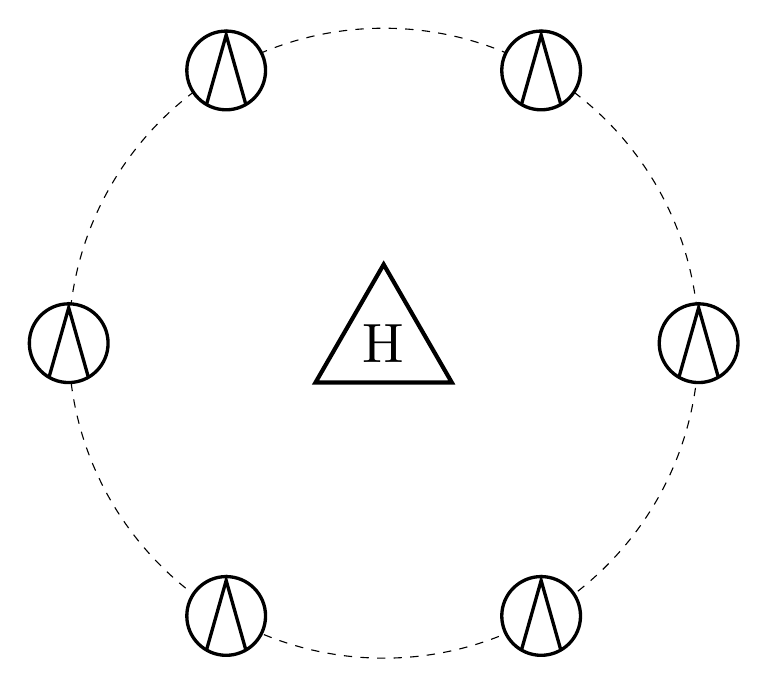
\begin{tikzpicture}
		\draw [dashed] (0,0) circle [radius=4];
		\epuck{4}{0}
		\epuck{2}{3.464}
		\epuck{-2}{3.464}
		\epuck{-4}{0}
		\epuck{-2}{-3.464}
		\epuck{2}{-3.464}
		
		\human{0}{0}
		%\draw (0,0) node[regular polygon,regular polygon sides=3,minimum height=2cm,minimum width=1cm,line width=1.5pt, draw] {\Huge{H}};
	\end{tikzpicture}
	\caption{Circle shape for the swarm to get the widest protected surface for a given amount of robots.}
	\label{fig:circle_shape}
	\end{figure}
	
		The figure \ref{fig:circle_shape} represents the kind of circle that we would like to get for 6 robots and 1 human in the centre.
		
	\section{State Machine}
	
	The final implementation is built on 2 layers. The upper layer is the state machine, having for each state a specific behaviour in the lower layer. Figure \ref{fig:state_machine} illustrates the whole structure of the upper layer. Only part of the states rely on virtual physics: \emph{Human} and \emph{Default}. The others simply link the sensor values to the wheels speed.\\
	
	The transitions without any number are taken without any condition, right after the corresponding behaviour has been applied (the time step period is over). One could see the 3 lowest states as sub-states of \emph{Normal}. At the beginning of each time step, if the controller is in the \emph{Normal} state, it has to choose between the 3 different sub-states. The conditions are listed with numbers in the figure \ref{fig:state_machine}.
	
	\begin{figure}[!h]\centering
		\begin{minipage}[c]{.49\textwidth}
			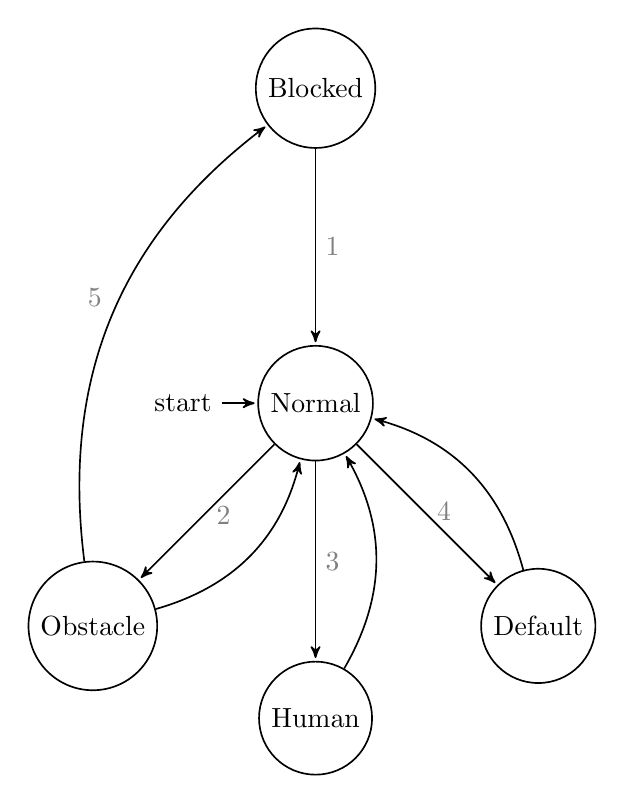
\begin{tikzpicture}[->, >=stealth', shorten >=1pt, auto, node distance=4cm, semithick]
				\node[initial,state] (NORMAL)                    {Normal};
		  		\node[state]         (OBS) [below left of=NORMAL] {Obstacle};
		  		\node[state]         (HU) [below of=NORMAL] {Human};
		  		\node[state]         (DEF) [below right of=NORMAL] {Default};
		  		\node[state]         (BLOCK) [above of=NORMAL]       {Blocked};
		  		
		  		\path	(BLOCK)		edge		node					{\color{gray} 1}	(NORMAL)
		  				(NORMAL)		edge		node[yshift=0.2cm]	{\color{gray} 2}	(OBS)
		  				(NORMAL)		edge		node					{\color{gray} 3}	(HU)
		  				(NORMAL)		edge		node	[yshift=-0.2cm]	{\color{gray} 4}	(DEF)
		  				(OBS)		edge		[bend left]	node		{\color{gray} 5}	(BLOCK)
		  				(OBS)		edge		[bend right]	node		{}				(NORMAL)
		  				(HU)			edge		[bend right]	node		{}				(NORMAL)
		  				(DEF)		edge		[bend right]	node		{}				(NORMAL);
			\end{tikzpicture}
%			
%			\begin{tikzpicture}[->, >=stealth', shorten >=1pt, auto, node distance=4cm, semithick]
%		  		\node[state]         (OBS)						{Obstacle};
%		  		\node[state]         (HU) [below of=OBS]	{Human};
%		  		\node[state]         (DEF) [below of=HU]		{Default};
%		  		\node[state]         (BLOCK) [right of=HU]{Blocked};
%		  		
%		  		\path	(OBS)		edge	[bend left]	node		{\color{gray} 1}	(BLOCK)
%		  				(OBS)		edge	[bend left]	node[yshift=-1cm]		{\color{gray} 2}				(DEF)
%		  				(OBS)		edge	[bend left]	node	[left]	{\color{gray} 3}				(HU)
%		  				(HU)			edge	[bend left]	node[right]		{\color{gray} 4}				(OBS)
%		  				(HU)			edge	[bend left]	node	[left]	{\color{gray} 2}				(DEF)
%		  				(DEF)		edge	[bend left]	node[right]		{\color{gray} 3}				(HU)
%		  				(DEF)		edge	[bend left]	node		{\color{gray} 4}				(OBS)
%		  				(BLOCK)		edge				node		{\color{gray} 5}				(OBS)
%		  				(BLOCK)		edge				node		{\color{gray} 6}				(HU)
%		  				(BLOCK)		edge				node		{\color{gray} 7}				(DEF);
%			\end{tikzpicture}
		\end{minipage}
		\hfill
		\begin{minipage}[c]{.49\textwidth}
%			\begin{enumerate}
%				\item Amount of direction change (left/right) while having an obstacle around reaches a threshold.
%				\item No human nor obstacle found.
%				\item Human found around the robot.
%				\item Obstacle around the robot.
%				\item No more obstacle in front but obstacle elsewhere.
%				\item No more obstacle in front \& human found.
%				\item No more obstacle in front \& no human nor obstacle.
%
%			\end{enumerate}

			\begin{enumerate}
				\item No more obstacle in front.
				\item Obstacle found around the robot.
				\item Human found around the robot.
				\item Neither of the previous criteria met.
				\item Amount of direction change (left/right) while having an obstacle around reaches a threshold.
			\end{enumerate}
		\end{minipage}
		
		\caption{State machine of the final behaviour.}
		\label{fig:state_machine}
	\end{figure}
	
	\section{Virtual Physics}
	
	Section \ref{sec:virtual_physics} explained how the laws of physics can be used to design a behaviour. Intuitively, this method seemed the most appropriate to create a behaviour whose main feature is a \enquote{protection barrier} around a human. When it comes to pattern creation, people usually first consider using repulsive and attractive forces to make the robots automatically adjust their position with respect to others.\\
	
	Indeed, the laws of physics force the system to get to a state of minimum energy, i.e., to reach a global minimum of the potential function of the system. Since the force is proportional to the derivative of the corresponding potential, the minimum of the potential function means the disappearance of the forces. For the forces to disappear, every robot needs to be at the desired location.
	
	$$\vec{f} = -\vec{\nabla}P$$, P being the system's potential. The following sections will explain in detail the different potentials that were implemented to obtain the desired behaviour.
	
		\subsection{Potentials}
		
		In this section, the potentials are grouped by states in which they are used. Since virtual physics are used in only 2 states, we have only 2 groups.
		
			\subsubsection{Human}
			
			The controller enters the \emph{Human} state at the beginning of the time step only if a human is found nearby. The complete potential for this state is the sum of 3 components: the \emph{human potential}, the \emph{gravity potential} and the \emph{agent repulsion potential}.
		
				\paragraph{Human Potential}
				
				\begin{figure}[!h]\centering
					\begin{tikzpicture}[xscale=0.2,yscale=0.2]
						\draw [<->] (0,5) -- (0,0) -- (40,0);
						\draw[blue,thick, domain=28:70] plot (\x, {-4*500/\x*((30/\x)^4-(30/\x)^2)});
					\end{tikzpicture}
				\end{figure}
				
				
				\paragraph{Gravity Potential}
				\paragraph{Agent Repulsion Potential}
			
			\subsubsection{Default}
		
	\section{E-pucks}
	
	\section{ARGoS}
	
	\section{Range and Bearing Sensor}
		\subsection{Tests}
		\subsection{Calibration}
		\subsection{Conclusions}

	\section{Omnidirectional Camera Sensor}
		\subsection{Tests}

	\section{The Hardware}
		\subsection{Objective}
		\subsection{Choices}
		\subsection{Blueprints}
		\subsection{Build Process}

\chapter{Assessments}
	\section{Tracking System}
	\section{Metrics}
	\section{More robots ?}
	\section{Tests Scenarios}
	\section{Human Travelling Speed ?}
	\section{Usability Study}

\chapter{Future Works}
	\section{Other Robots}
	\section{Human Guidance}
		\subsection{Zero Visibility Areas or Blind People}
		\subsection{Human Motion Synchronisation}
		\subsection{Vehicle Guidance}

\chapter{Acknowledgements}

[Never gonna give you up\\
Never gonna let you down\\
Never gonna run around and desert you\\
Never gonna make you cry\\
Never gonna say goodbye\\
Never gonna tell a lie and hurt you]

\newpage

%%%%%%%%%%%%%%%%%%%%%%%%%%%%%%%%%%%%%%%%%%%%%%%%%%%%%%%
% BIBLIOGRAPHY
%%%%%%%%%%%%%%%%%%%%%%%%%%%%%%%%%%%%%%%%%%%%%%%%%%%%%%%

\begin{filecontents}{thesis.bib}
%http://en.wikibooks.org/wiki/LaTeX/Bibliography_Management

@inproceedings{podevijn2012self,
  title={Self-organised feedback in human swarm interaction},
  author={Podevijn, Ga{\"e}tan and O’Grady, Rehan and Dorigo, Marco},
  booktitle={Proceedings of the workshop on robot feedback in human-robot interaction: how to make a robot readable for a human interaction partner (Ro-Man 2012)},
  year={2012}
}

@incollection{podevijn2014gesturing,
  title={Gesturing at subswarms: Towards direct human control of robot swarms},
  author={Podevijn, Ga{\"e}tan and O’Grady, Rehan and Nashed, Youssef SG and Dorigo, Marco},
  booktitle={Towards Autonomous Robotic Systems},
  pages={390--403},
  year={2014},
  publisher={Springer}
}

@article{brambilla2013swarm,
  title={Swarm robotics: a review from the swarm engineering perspective},
  author={Brambilla, Manuele and Ferrante, Eliseo and Birattari, Mauro and Dorigo, Marco},
  journal={Swarm Intelligence},
  volume={7},
  number={1},
  pages={1--41},
  year={2013},
  publisher={Springer}
}

@incollection{csahin2005swarm,
  title={Swarm robotics: From sources of inspiration to domains of application},
  author={{\c{S}}ahin, Erol},
  booktitle={Swarm robotics},
  pages={10--20},
  year={2005},
  publisher={Springer}
}

@phdthesis{kazadi2000swarm,
  title={Swarm engineering},
  author={Kazadi, Sanza T},
  year={2000},
  school={California Institute of Technology}
}

@book{minsky1967computation,
  title={Computation: finite and infinite machines},
  author={Minsky, Marvin L},
  year={1967},
  publisher={Prentice-Hall, Inc.}
}

@article{granovetter1978threshold,
  title={Threshold models of collective behavior},
  author={Granovetter, Mark},
  journal={American journal of sociology},
  pages={1420--1443},
  year={1978},
  publisher={JSTOR}
}

@inproceedings{bonabeau1997adaptive,
  title={Adaptive Task Allocation Inspired by a Model of Division of Labor in Social Insects.},
  author={Bonabeau, Eric and Sobkowski, Andrej and Theraulaz, Guy and Deneubourg, Jean-Louis},
  booktitle={BCEC},
  pages={36--45},
  year={1997}
}

@article{bachrach2010composable,
  title={Composable continuous-space programs for robotic swarms},
  author={Bachrach, Jonathan and Beal, Jacob and McLurkin, James},
  journal={Neural Computing and Applications},
  volume={19},
  number={6},
  pages={825--847},
  year={2010},
  publisher={Springer}
}

@article{wolpert1999introduction,
  title={An introduction to collective intelligence},
  author={Wolpert, David H and Tumer, Kagan},
  journal={arXiv preprint cs/9908014},
  year={1999}
}

@article{abbott2006emergence,
  title={Emergence explained: Abstractions: Getting epiphenomena to do real work},
  author={Abbott, Russ},
  journal={Complexity},
  volume={12},
  number={1},
  pages={13--26},
  year={2006},
  publisher={Wiley Online Library}
}

@article{pinciroli2012argos,
  title={ARGoS: a modular, parallel, multi-engine simulator for multi-robot systems},
  author={Pinciroli, Carlo and Trianni, Vito and O’Grady, Rehan and Pini, Giovanni and Brutschy, Arne and Brambilla, Manuele and Mathews, Nithin and Ferrante, Eliseo and Di Caro, Gianni and Ducatelle, Frederick and others},
  journal={Swarm intelligence},
  volume={6},
  number={4},
  pages={271--295},
  year={2012},
  publisher={Springer}
}

@inproceedings{daily2003world,
  title={World embedded interfaces for human-robot interaction},
  author={Daily, Mike and Cho, Youngkwan and Martin, Kevin and Payton, Dave},
  booktitle={System Sciences, 2003. Proceedings of the 36th Annual Hawaii International Conference on},
  pages={6--pp},
  year={2003},
  organization={IEEE}
}

@incollection{baizid2009human,
  title={Human multi-robots interaction with high virtual reality abstraction level},
  author={Baizid, Khelifa and Li, Zhao and Mollet, Nicolas and Chellali, Ryad},
  booktitle={Intelligent Robotics and Applications},
  pages={23--32},
  year={2009},
  publisher={Springer}
}

@inproceedings{mclurkin2006speaking,
  title={Speaking Swarmish: Human-Robot Interface Design for Large Swarms of Autonomous Mobile Robots.},
  author={McLurkin, James and Smith, Jennifer and Frankel, James and Sotkowitz, David and Blau, David and Schmidt, Brian},
  booktitle={AAAI Spring Symposium: To Boldly Go Where No Human-Robot Team Has Gone Before},
  pages={72--75},
  year={2006}
}


\end{filecontents}

\nocite{*}
\bibliographystyle{plainnat}
\bibliography{thesis}

\end{document}
